
\paragraph{VQVAE}\mbox{}
\subparagraph{Configuration}\mbox{}\\

\begin{table}[h!]
\centering
\begin{tabular}{|l|l|}
\hline
\textbf{Parameter} & \textbf{Value} \\
\hline
\multicolumn{2}{|c|}{\textbf{Training}} \\
\hline
Accelerator & GPU \\
\hline
Devices & 2 \\
\hline
Precision & 32 \\
\hline
Strategy & DDP \\
\hline
Maximum Epochs & 10001 \\
\hline
\multicolumn{2}{|c|}{\textbf{Model}} \\
\hline
Input Channels & 1 \\
\hline
Output Channels & 1 \\
\hline
Embedding Channels & 8 \\
\hline
Number of Embeddings & 16384 \\
\hline
Spatial Dimensions & 3 \\
\hline
Hidden Channels & [32, 64, 128, 256] \\
\hline
Kernel Sizes & [3, 3, 3, 3] \\
\hline
Strides & [1, 2, 2, 2] \\
\hline
Embedding Loss Weight & 1 \\
\hline
Beta & 1 \\
\hline
Loss Function & L1 \\
\hline
Deep Supervision & 0 \\
\hline
Use Attention & [False, False, True, True] \\
\hline
Normalization & Group (num\_groups: 4, affine: True) \\
\hline
Sample Every N Epochs & 20 \\
\hline
Learning Rate & 5e-6 \\
\hline
\multicolumn{2}{|c|}{\textbf{Dataset}} \\
\hline
Caching & Disk \\
\hline
Path & /ravana/d3d\_work/micorl/data/ct\_images\_prostate\_32fixed/ \\
\hline
Image Size & 128 \\
\hline
Number of Slices & 32 \\
\hline
Window Width & 400 \\
\hline
Window Level & 60 \\
\hline
\end{tabular}
\caption{Configuration of the VQVAE approach.}
\label{table:training_params}
\end{table}

\subparagraph{Training}\mbox{}\\

The model was trained for 10000 epochs. As visible in the plots below, all losses started to slow down after epoch 2000. 

\begin{figure}[H]
\minipage{0.49\textwidth}
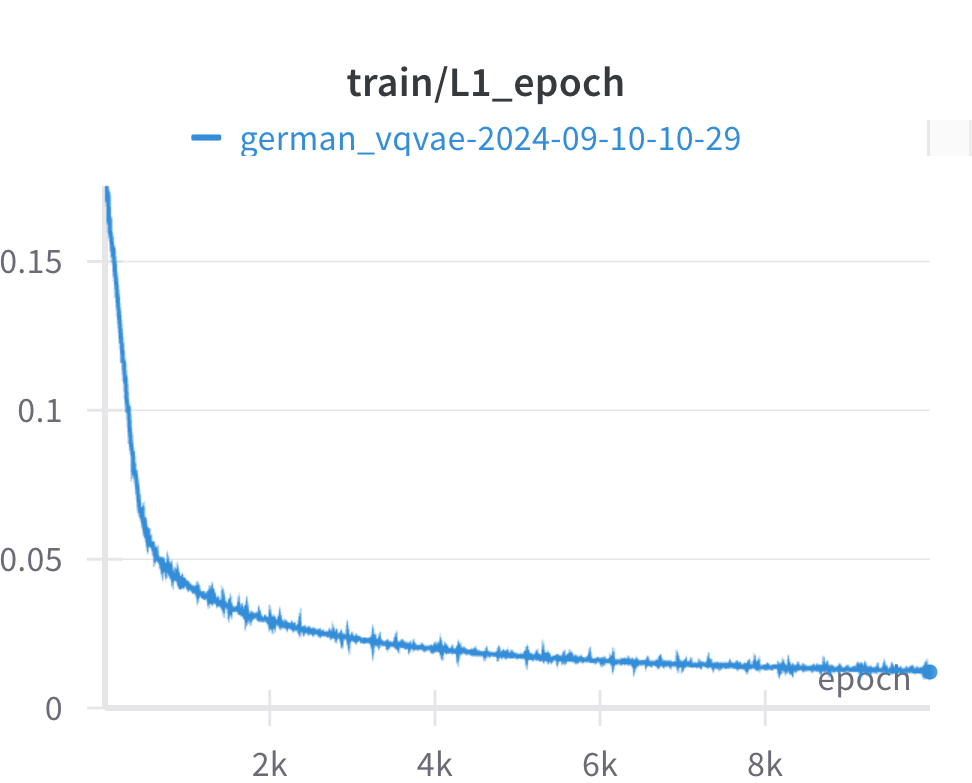
\includegraphics[width=\linewidth]{detailed_engineering/German VQVAE/charts/train_l1.png}
\caption{Training.}
\endminipage\hfill
\minipage{0.49\textwidth}
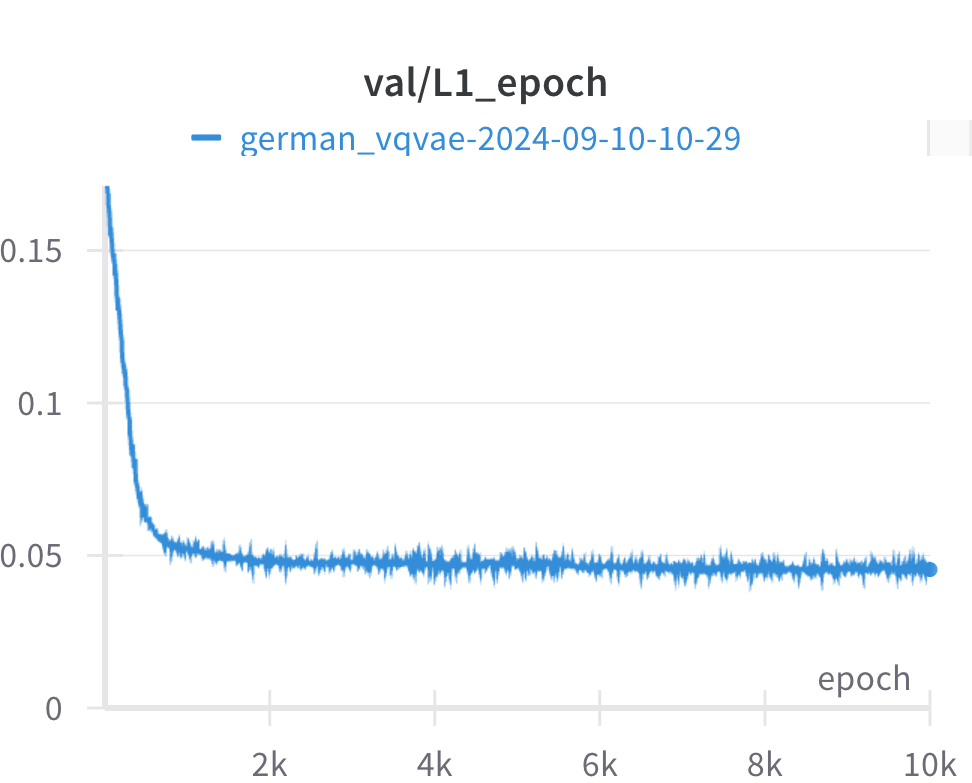
\includegraphics[width=\linewidth]{detailed_engineering/German VQVAE/charts/val_l1.png}
\caption{Validation.}
\endminipage
\caption{L1 loss between input and its reconstruction. Lower is better.}
\end{figure}

\begin{figure}[H]
\minipage{0.49\textwidth}
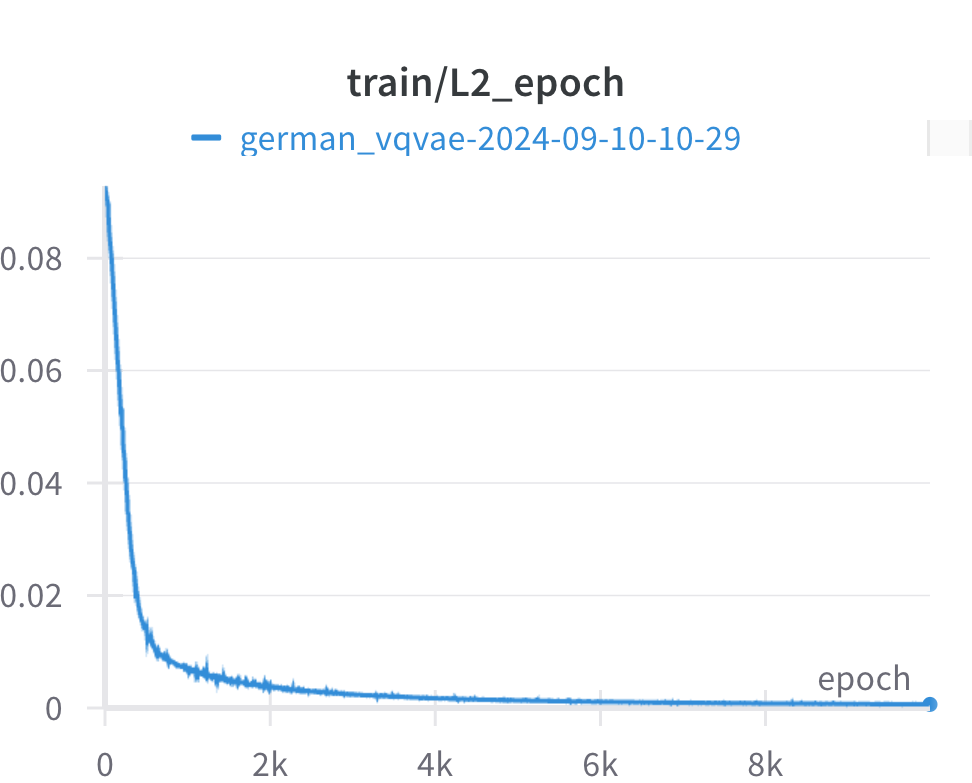
\includegraphics[width=\linewidth]{detailed_engineering/German VQVAE/charts/train_l2.png}
\caption{Training.}
\endminipage\hfill
\minipage{0.49\textwidth}
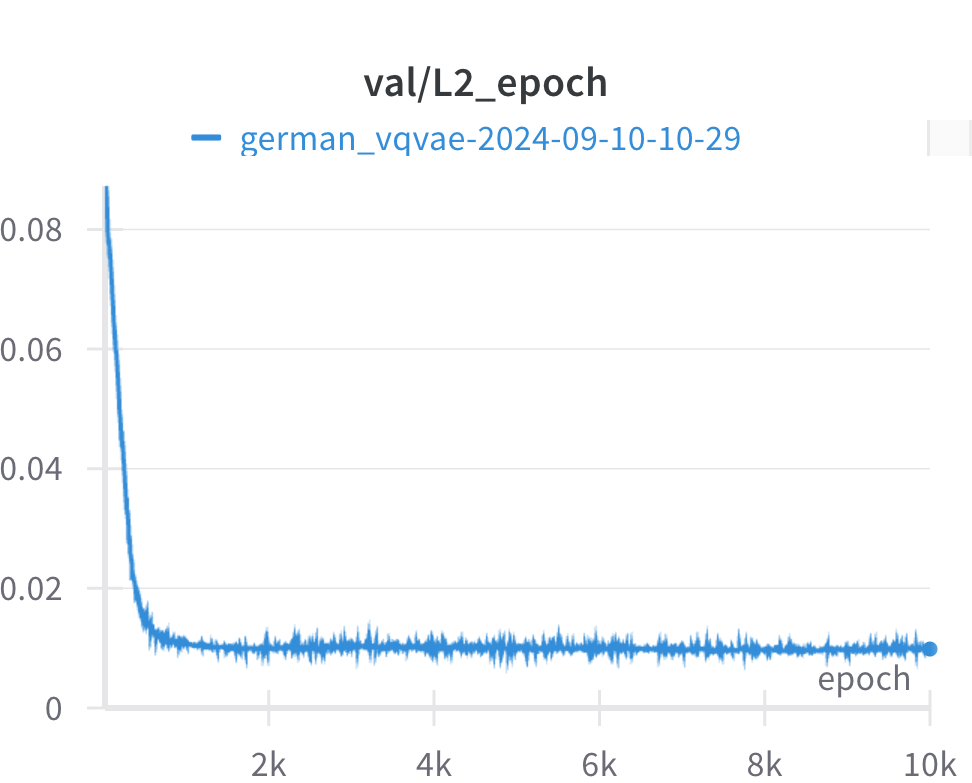
\includegraphics[width=\linewidth]{detailed_engineering/German VQVAE/charts/val_l2.png}
\caption{Validation.}
\endminipage
\caption{L2 loss between input and its reconstruction. Lower is better.}
\end{figure}

\begin{figure}[H]
\minipage{0.49\textwidth}
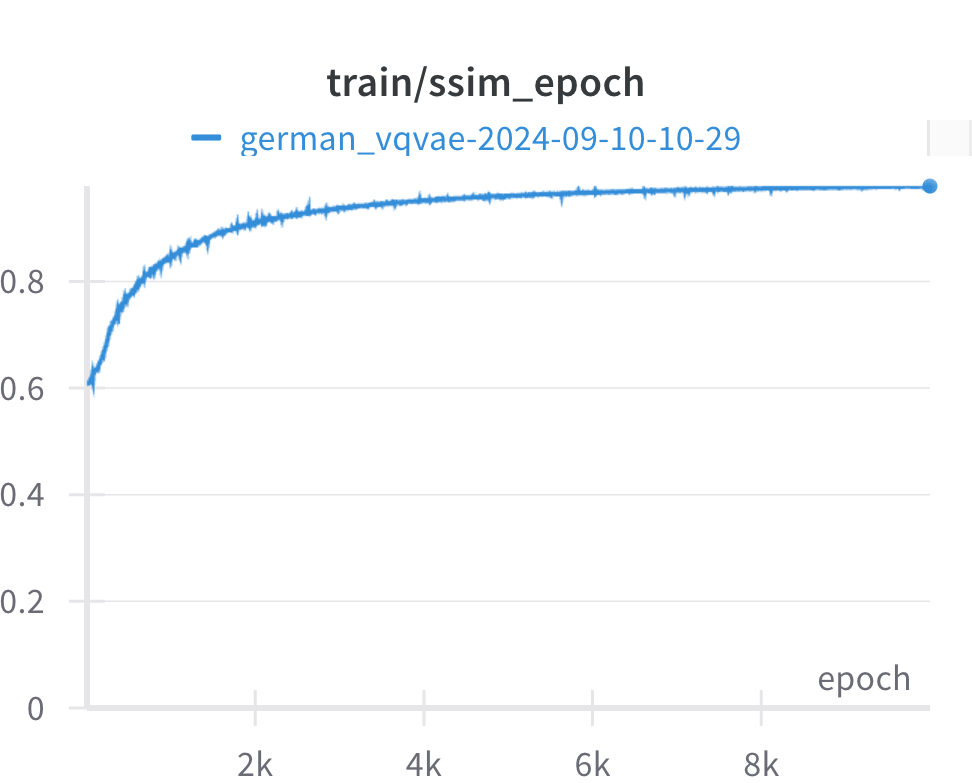
\includegraphics[width=\linewidth]{detailed_engineering/German VQVAE/charts/train_ssim.png}
\caption{Training.}
\endminipage\hfill
\minipage{0.49\textwidth}
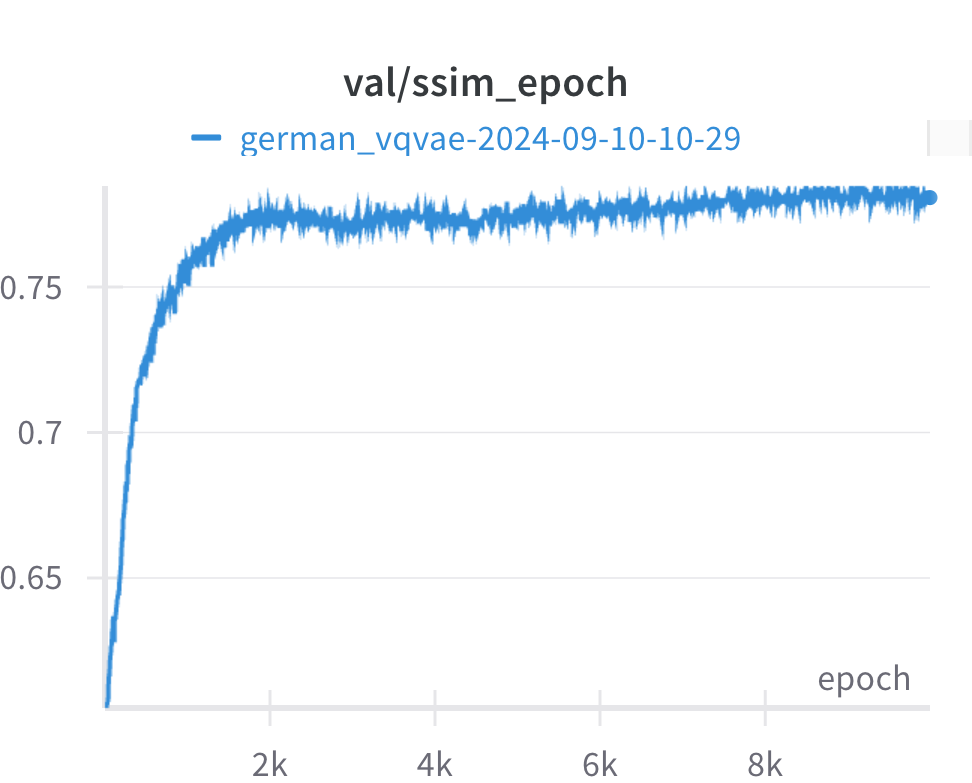
\includegraphics[width=\linewidth]{detailed_engineering/German VQVAE/charts/val_ssim.png}
\caption{Validation.}
\endminipage
\caption{SSIM loss between input and its reconstruction. Higher is better.}
\end{figure}




\subparagraph{Results}\mbox{}\\

The best results were obtained for a checkpoint of the model from the 8499 epoch. At that point, model reconstructions seem almost indistinguishable from the original, as is shown in the figure \ref{fig:german_vqvae_best}.

\begin{figure}[H]
    \centering
    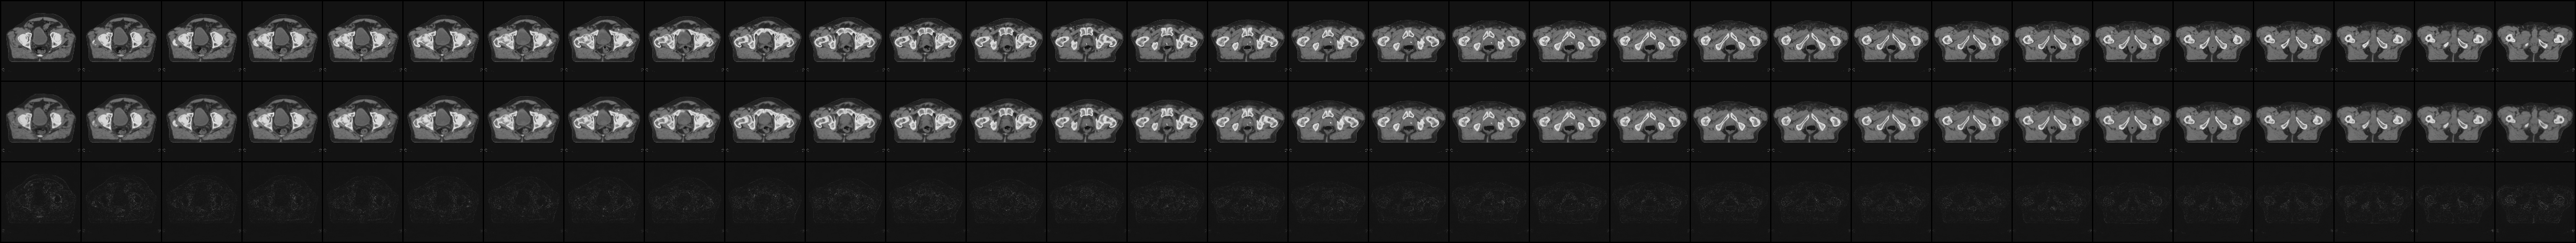
\includegraphics[width=\linewidth]{detailed_engineering/German VQVAE/charts/best_german_vqvae.png}
    \caption{The best quality reconstruction achieved. Epoch 8499, step 10540. Top - input, middle - reconstruction, bottom their difference}
    \label{fig:german_vqvae_best}
\end{figure}

